
\documentclass[
    article, 
    12pt,				% tamanho da fonte
	oneside,			% para impressão apenas no recto. Oposto a twoside
	a4paper,			% tamanho do papel. 
	% -- opções da classe abntex2 --
	chapter=TITLE,		% títulos de capítulos convertidos em letras maiúsculas
	section=TITLE,		% títulos de seções convertidos em letras maiúsculas
	%subsection=TITLE,	% títulos de subseções convertidos em letras maiúsculas
	%subsubsection=TITLE % títulos de subsubseções convertidos em letras maiúsculas
	% -- opções do pacote babel --
	english,			% idioma adicional para hifenização
	english,				% o último idioma é o principal do documento
	sumario=tradicional
]{abntex2}

\usepackage[alf]{abntex2cite}

\usepackage{graphicx,url}
% \usepackage[USenglish,brazil]{babel}   
\usepackage[utf8]{inputenc}
\usepackage{lmodern}			% Usa a fonte Latin Modern
\usepackage[T1]{fontenc}		% Selecao de codigos de fonte.
\usepackage{indentfirst}		% Indenta o primeiro parágrafo de cada seção.
\usepackage{nomencl} 			% Lista de simbolos
\usepackage{color}				% Controle das cores
\usepackage{microtype} 			% para melhorias de justificação
\usepackage[english,hyperpageref]{backref}	 % Paginas com as citações na bibl
\usepackage{helvet}             % Fonte Helvica - Arial

\renewcommand{\familydefault}{\sfdefault}    % set the default font as serif, i.e., Arial
     
% ---
% compila o indice
% ---
\makeindex
% ---

% ---
% Altera as margens padrões
% ---
\setlrmarginsandblock{2.54cm}{2.54cm}{*}
\setulmarginsandblock{2.44cm}{2.54cm}{*}
\checkandfixthelayout
% ---

% --- 
% Espaçamentos entre linhas e parágrafos 
% --- 

% O tamanho do parágrafo é dado por:
\setlength{\parindent}{1cm}

% Controle do espaçamento entre um parágrafo e outro:
\setlength{\parskip}{0.2cm}  % tente também \onelineskip

% Espaçamento simples
\SingleSpacing


% Remove espaçamento do resumo
\setlength\absleftindent{0cm}
\setlength\absrightindent{0cm}
% Garante que a fonte do texto do abstract será a mesma do documento, pois
% na classe memoir está \small
\renewcommand{\abstracttextfont}{\normalfont\normalsize}

\setlength{\footmarkwidth}{1.8em}
\setlength{\footmarksep}{-\footmarkwidth}
\setlength{\footparindent}{1em}

% Define como negrito usando tamanho normal das fontes na seção e capítulo
\renewcommand{\ABNTEXchapterfont}{\bfseries}

% Define a subseção como negrito e tamanho normal
\renewcommand{\ABNTEXsubsectionfont}{\bfseries}
\renewcommand{\ABNTEXsubsectionfontsize}{\normalsize}

% Define a seção terciária como itálico e tamanho normal
\renewcommand{\ABNTEXsubsubsectionfont}{\itshape}
\renewcommand{\ABNTEXsubsubsectionfontsize}{\normalsize}

\renewcommand{\ABNTEXsectionfontsize}{\normalsize}
\renewcommand{\ABNTEXchapterfontsize}{\normalsize}

\bibliographystyle{./references/abnt-bib}

\date{November 16, 2021}

\renewcommand{\imprimirautor}{
  \begin{flushright}
   \theauthor
   \footnote{Student of the computer science course at La Salle University - Unilasalle, enrolled in the database architecture course under the guidance of Prof. Aline Duarte Riva. E-mail: davi.201810357@unilasalle.edu.br. Date of submission: \thedate }
  \end{flushright}
}


\title{ \textbf{\uppercase{Ethereum: a distributed key value state machine}}}

\autor{
Davi F. Henrique
}

\begin{document} 

\selectlanguage{english}

\thetitle

\imprimirautor

\citeoption{ABNT-final}

\begin{resumo}
 The Ethereum has been adopted for decentralized blockchain applications, being used in other areas than decentralized finances.
 Allowing a new universe of peer to peer interactions, in a secure, scalable way.
 In this paper we covered about Ethereum, how the trilemma of scalability, security and decentralization is addressed.
 Focussing on the database concepts involving the implementation of the protocol, such as how the consensus is made, how the data is stored in the blockchain, how the transaction mechanism work.
 In order to better illustrate the concepts, we modeled a real estate application for the Ethereum blockchain platform by using Web3 components and concepts.
 
 \vspace{\onelineskip}
 Keywords: Smart Contract, Solidity, DeFi, NFT
\end{resumo}


\section{Introduction}

The concept of decentralized databases has been around for decades.
Wei Dai, in 1998, introduced the idea of creating money by solving computational puzzles, but the approach wasn't described in details such as how the decentralized consensus could be implemented.
The concept of "reusable proofs of work" emerged in 2005 from Hal Finney, by using the ideas from Wei Dai to create a concept for a cryptocurrency. 
The system fell short due to relying on trusted computing as a backend \cite{buterin_eth_whitepaper_2013}.

Decentralized currencies require decentralized consensus, which has been addressed in researches prior to the Bitcoin paper.
However, the protocols only solved the problem, known as the \textit{trilemma} of security, scalability and security in a partial manner.
By assuming that all participants are known, and produced security margins, which in anonymous setting are vulnerable to Sybil attacks \cite{buterin_eth_whitepaper_2013}.

The Bitcoin paper published by \citeauthor{nakamoto_bitcoin_2008} combined a simple decentralized consensus protocol, based on nodes grouping transactions into a block which is created every ten minutes.
Because the protocol uses proof of work, nodes with more computational power have more influence in the system.
It's more difficult to have more computational power than the network, comparing to simulating a million of nodes \cite{buterin_eth_whitepaper_2013}.

Besides the simplicity, Bitcoin was the first decentralized global ledger to become widely adopted \cite{wood_ethereum_2021}.
Being a foundation for other projects and cryptocurrencies, known as alternative coins, such as Litecoin and Primecoin.
There were projects that repurposed the mechanism of the protocol to beyond a cryptocurrency, such as Namecoin which aims to provide a decentralized name-resolution system \cite{wood_ethereum_2021}.  


\section{Ethereum}

Ethereum was proposed in \citeyear{buterin_eth_whitepaper_2013} by \citeauthor{buterin_eth_whitepaper_2013} as an open-source project with the intent of allowing the development of arbitrary consensus based applications, that have scalability, standardization, ease of development and interoperability. 
With a Turing-complete script language, which allows the creation of smart contracts, with arbitrary rules, state transition functions and transaction formats \cite{buterin_eth_whitepaper_2013}.
Ethereum was announced at The North American Bitcoin Conference in Miami, in 2014.
Having the first version launched in 2015, mainly for mining Ether and the test of decentralized applications \cite{eth_history_jianing_2021}. 

The system can be viewed as a database, a state machine with a transaction system in which transitions are executed incrementally.
Transactions are grouped into blocks, which are chained together in a chronological fashion, using a cryptographic hash function, that can be used as a reference for each block.
Because each transaction is registered in a chronological order, the block acts as a journal, allowing a history view of the global state.

Due to the decentralization, any participant in the system can create a new block on some older block that exists.
This implies that in a given time, multiple states of the system may coexist: some nodes believing that a particular path is the canonical, others believing other path with different blocks.
The resulting data structure is a tree of blocks. 
In order to form an agreement upon which path is canonical, to generate a consensus, a simplified version of the GHOST algorithm is used, more detailed in \autoref{sec:consensus} \cite{wood_ethereum_2021}.


\section{Accounts}

There are two types of accounts, External Owned Account (EOA) and Contract Account.
External Owned Accounts are controlled by private keys, Contract Accounts are controlled by their contract code.
EOA doesn't contain contract code, but can be used to create a contract account, the act of deploying a smart contract.
Each account has a 20 byte address and state transitions \cite{wood_ethereum_2021}. 
An account has four fields:

\begin{alineas}
    \item Nonce. 
    The number of transactions sent from this address or, in case of a contract account, the number of contract creations made by this account.
    The main purpose of this field is to make sure each transaction is processed once. 
    
    \item Balance. 
    The current balance of the account, expressed in Wei.
    
    \item Storage root.
    A hash of the root node of the tree that store the storage of this account.
    
    \item Code hash.
    A hash of the EVM code of this account, if it's a contract account.
    This is the only immutable field.
\end{alineas}

Whenever one transaction issued by the account is processed, the nonce is incremented, the balance change when Ether is transferred, but for a contract account the code hash is immutable.
That is, after the deployment of a smart contract, its code can't be changed.
This arises the importance of good software engineering practices such as automated testing to prevent faulty software.
The concept of upgradable smart contracts exists and allows the change of a contract code by using a proxy mechanism \cite{openzeppelin_proxy_upgrade}.

The \autoref{fig:ethereum_account_state} illustrate the account state with the fields and the storage trie.

\begin{figure}[ht]
    \centering
    \caption{Ethereum account state}
    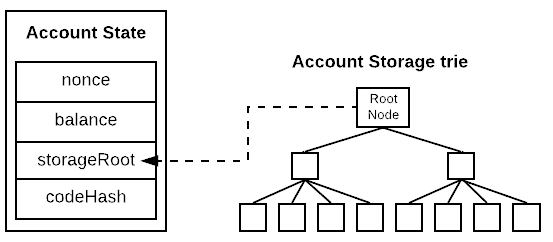
\includegraphics[width=300px]{images/Account-state.png}
    \fonte{\citeonline{saldanha_ethereum_merkle_2018}}
    \label{fig:ethereum_account_state}
\end{figure}


\section{Messages and transactions}

A transaction is an instruction cryptographically signed by an external owned account. 
The sender of a transaction can not be a contract account.
There are two types of transactions, those who creates a new contract account with associated code and those which result in message calls \cite{wood_ethereum_2021}.
A transaction has the given fields:

\begin{alineas}
  \item Nonce. The number of transactions sent by the sender.
  \item Gas price. The price expressed in Wei to pay per unit of gas used by all computation and storage costs of this transaction.
  \item Gas limit. The maximum amount of gas that should be used during the execution of this transaction.
  \item To. The address (20 bytes identifier) of the message recipient, or 0 in case of a contract creation.
  \item Value. The number of Wei to be transferred to the message recipient.
  \item v, r and s. Values used to determine the sender of the transaction.
  \item Init. The EVM code fragment for the account initialization, in case of an account creation.
\end{alineas}

In order to prevent infinite loops in the execution of a transaction, it's required to set the limit of gas that can be used.
It's possible to call, in a read only manner, a contract account to retrieve data or to simulate a transaction \footnote{https://web3js.readthedocs.io/en/v1.2.9/web3-eth.html?highlight=call\#call}.
This transaction doesn't cost Ether and is executed locally in the node that receives it, but it's not broadcasted in the network to be included in a new block.
The changes are discarded when the execution of the transaction is finished and the returned value of the function called is returned.

\section{Storage}

The world state is not stored on the blockchain, it's a key value structure which maps address (20 bytes identifiers) to account states.
This mapping is expected to be implemented using a modified Merkle Patricia tree, requiring a simple key value database that maps byte arrays to byte arrays \cite{wood_ethereum_2021}.
There are client implementations that make use of Leveldb or Rocksdb for the storage of the world state \cite{ethereum_data_structure_jezek_2021}.

The Merkle tree is a data structure designed for fast verification of data consistency by using cryptographic hash functions, such as SHA 256. 
Every node of the tree contains in its hash the hash of its children.
The main advantage of this tree in a distributed environment, is the ability to verify the consistency of a data set without the necessity of exchanging the data itself, but only relaying on its hash generated \cite{ethereum_data_structure_jezek_2021}.

The Merkle Patricia tree is a data structure that combines the concepts of the Merkle tree and the Patricia tree, a tree where the data is represented by a table, where columns are nodes and rows are branches \cite{ethereum_data_structure_jezek_2021}.
The tree stores the primary keys while grouping by their common paths in one node.
Defining three types of nodes with a specific structure:

\begin{alineas}
    \item Branch. Contains 17 items.
    \item Extension. Contains 2 items.
    \item Leaf. Contains 2 items.
\end{alineas}


\begin{figure}[ht]
    \centering
    \caption{Ethereum's storage overview}
    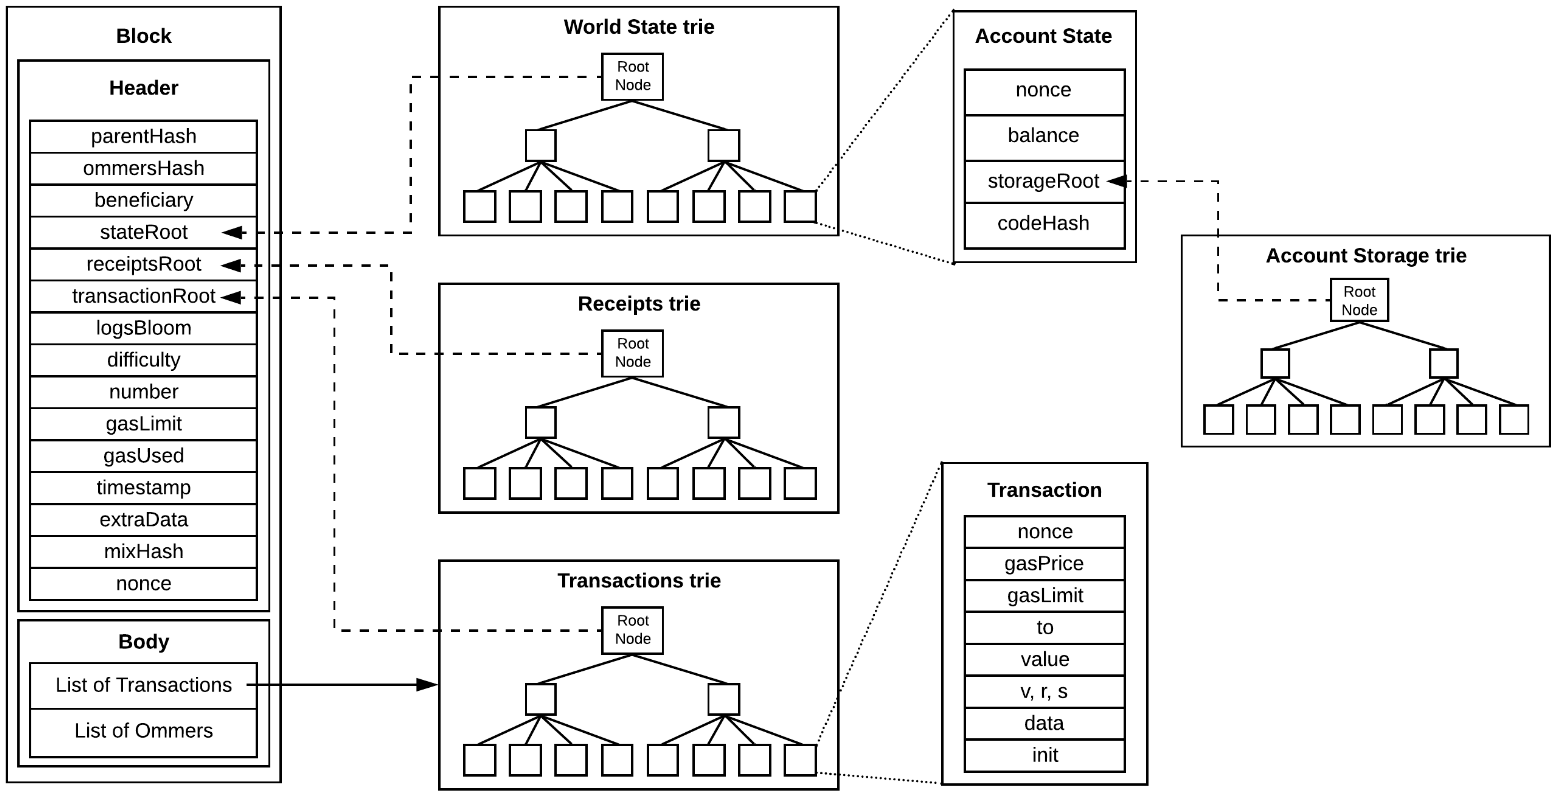
\includegraphics[width=\textwidth]{images/ethereu_storage_overview.png}
    \fonte{\citeonline{saldanha_ethereum_merkle_2018}}
    \label{fig:ethereum_storage_overview}
\end{figure}


\section{Ethereum virtual machine}

The code for an Ethereum contract is written in a low-level byte-code language which is stack-based, referred to as EVM code.
The Ethereum virtual machine has a simple architecture which is stack based and has a 256 bit word size, but doesn't follow the von Neumann standard.
The memory model is a simple word addressable byte array, having the maximum of 1024 items on the stack \cite{wood_ethereum_2021}.
The machine has a storage model which is independent, having a word addressable word array, and it's not volatile.

\begin{figure}[ht]
    \centering
    \caption{Ethereum virtual machine architecture}
    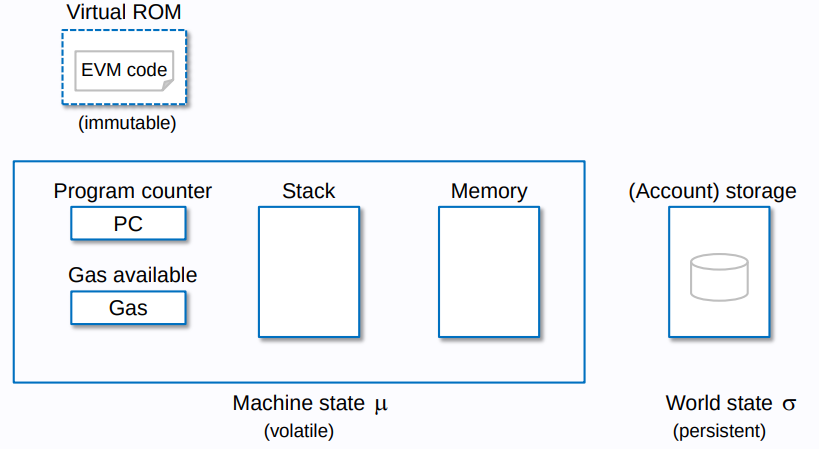
\includegraphics[width=370px]{images/evm_architecture.png}
    \fonte{\citeonline[p. 48]{takenobu_evm_ilustred}}
    \label{fig:evm_architecture}
\end{figure}

The program code consists of operations encoded into bytes and is stored into a virtual ROM, being only accessible through a specialized instruction \cite{wood_ethereum_2021}.
The code can access the block header data, the sender and the data of the incoming message and can return a byte array as output.

The code execution can be viewed as an infinite loop that consists of executing the current operation of the program counter, then incrementing it, until the end of the code is reached or STOP or RETURN instruction is detected \cite{buterin_eth_whitepaper_2013}.
When there is an exception, such as out of gas exception, the machine is halted and the changes made to the state during code execution are discarded \cite{wood_ethereum_2021}.

\subsection{Solidity}

Solidity\footnote{https://docs.soliditylang.org/en/v0.8.10/} is a high-level object-oriented programming language for implementing smart contracts.
The language uses curly brackets and is influenced by C++, Python, Javascript, having the Ethereum machine as the target.
Solidity supports inheritance, libraries, user-defined types, allowing the flexible creation of smart contracts and the reusability of the code.

In Solidity, variables can be specified to be stored on memory or on the state.
The state variables of contracts are stored in a compact way which can group multiple variables values into the same storage slot.
Starting from slot 0, data is stored into a contiguous way, item after item, considering the size of each value\footnote{https://docs.soliditylang.org/en/v0.8.10/internals/layout\_in\_storage.html}.

\section{Consensus} \label{sec:consensus}

Ethereum uses a simplified version of the Greedy Heaviest-Observed Sub-Tree (GHOST) consensus protocol \cite{ghost_sompolinsky_2015}, which only goes down five levels \cite{buterin_eth_whitepaper_2013}.
GHOST uses a different mechanism to select the main chain, comparing to the Bitcoin longest chain introduced by \citeauthor{nakamoto_bitcoin_2008}.
The algorithm selects the path which has the most computation done upon it, or the heaviest path.
Using the criteria of the largest subtree by cardinality.
The block number of the leaf, which is the number of blocks, helps to determine the main chain. 

\begin{figure}[ht]
    \centering
    \caption{Blockchain tree path selected by GHOST}
    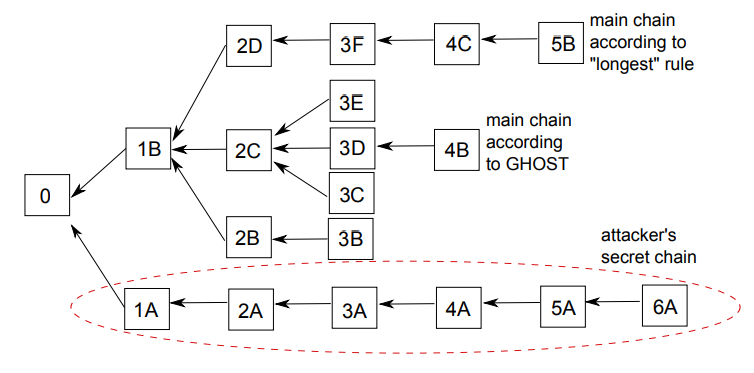
\includegraphics[width=\textwidth]{images/ghost_tree.png}
    \fonte{\citeonline[p. 8]{ghost_sompolinsky_2015}}
    \label{fig:blockchain_tree}
\end{figure}

In the \autoref{fig:blockchain_tree} an attacker tries to manipulate the transactions in an honest network by mining fraudulent blocks. 
The main chain selected wasn't the longest chain, but the one that the subtree has more cardinality. 

When the Ethereum protocol change, there might be a permanent fork in the network due to actors not agreeing about the change.
To distinguish between diverged blockchains, the Ethereum improvement proposal 155 by Buterin introduced the concept of chain ID \cite{wood_ethereum_2021}.


\section{Use cases}

Ethereum can be used as a platform for a variety of real-world applications, beyond a financial system, which includes insurance, real estate, cloud computing. Ethereum can be used for:

\begin{alineas}
    \item Decentralized Autonomous Organizations (DAO). 
    Community driven organizations, governed by rules coded in software, where administrative decisions are voted by the community.
    DAOs were one of the innovations that Ethereum made possible.
    
    \item Token systems; arts marketplace.
    A marketplace of art where art can be sold with unique guaranties, such as authenticity, owner verification.
    By using the non-fungible token (NFT) which is unique, indivisible, it's possible to store the digital asset in a secure and transferrable way.
    NFT is another innovation possible due to Ethereum.
\end{alineas}

Ethereum is not suitable for real time, low latency applications such as monitoring vehicle speed.
Due to the gas constraint, it's not recommended to store large binary data such as images, documents, videos, files.
Usually another solution such as IPFS is used to address this necessity \cite{ethereum_data_store_kostamis_2021}.


\section{Real estate application}

The real estate application is a Web application where realtors can register real estates for sale.
The application has a real estate catalog where buyers can search by place, pricing, trading options.
The system notifies realtors about outdated records and buyers interested in real estates.

The core functionality of the application is implemented in smart contracts by using the programming language Solidity. 
To support a better search mechanism for data stored by the smart contracts, we used the Graph\footnote{https://thegraph.com/docs/about/introduction}, a decentralized protocol for indexing and querying data from Ethereum.
The images are stored in a IPFS node and only the URL of the image is stored on the blockchain.

The project source code is stored in a public GitHub repository\footnote{https://github.com/dangerousplay/real-estate-dapp} and can be executed locally.


\begin{figure}[ht]
    \centering
    \caption{Application architecture}
    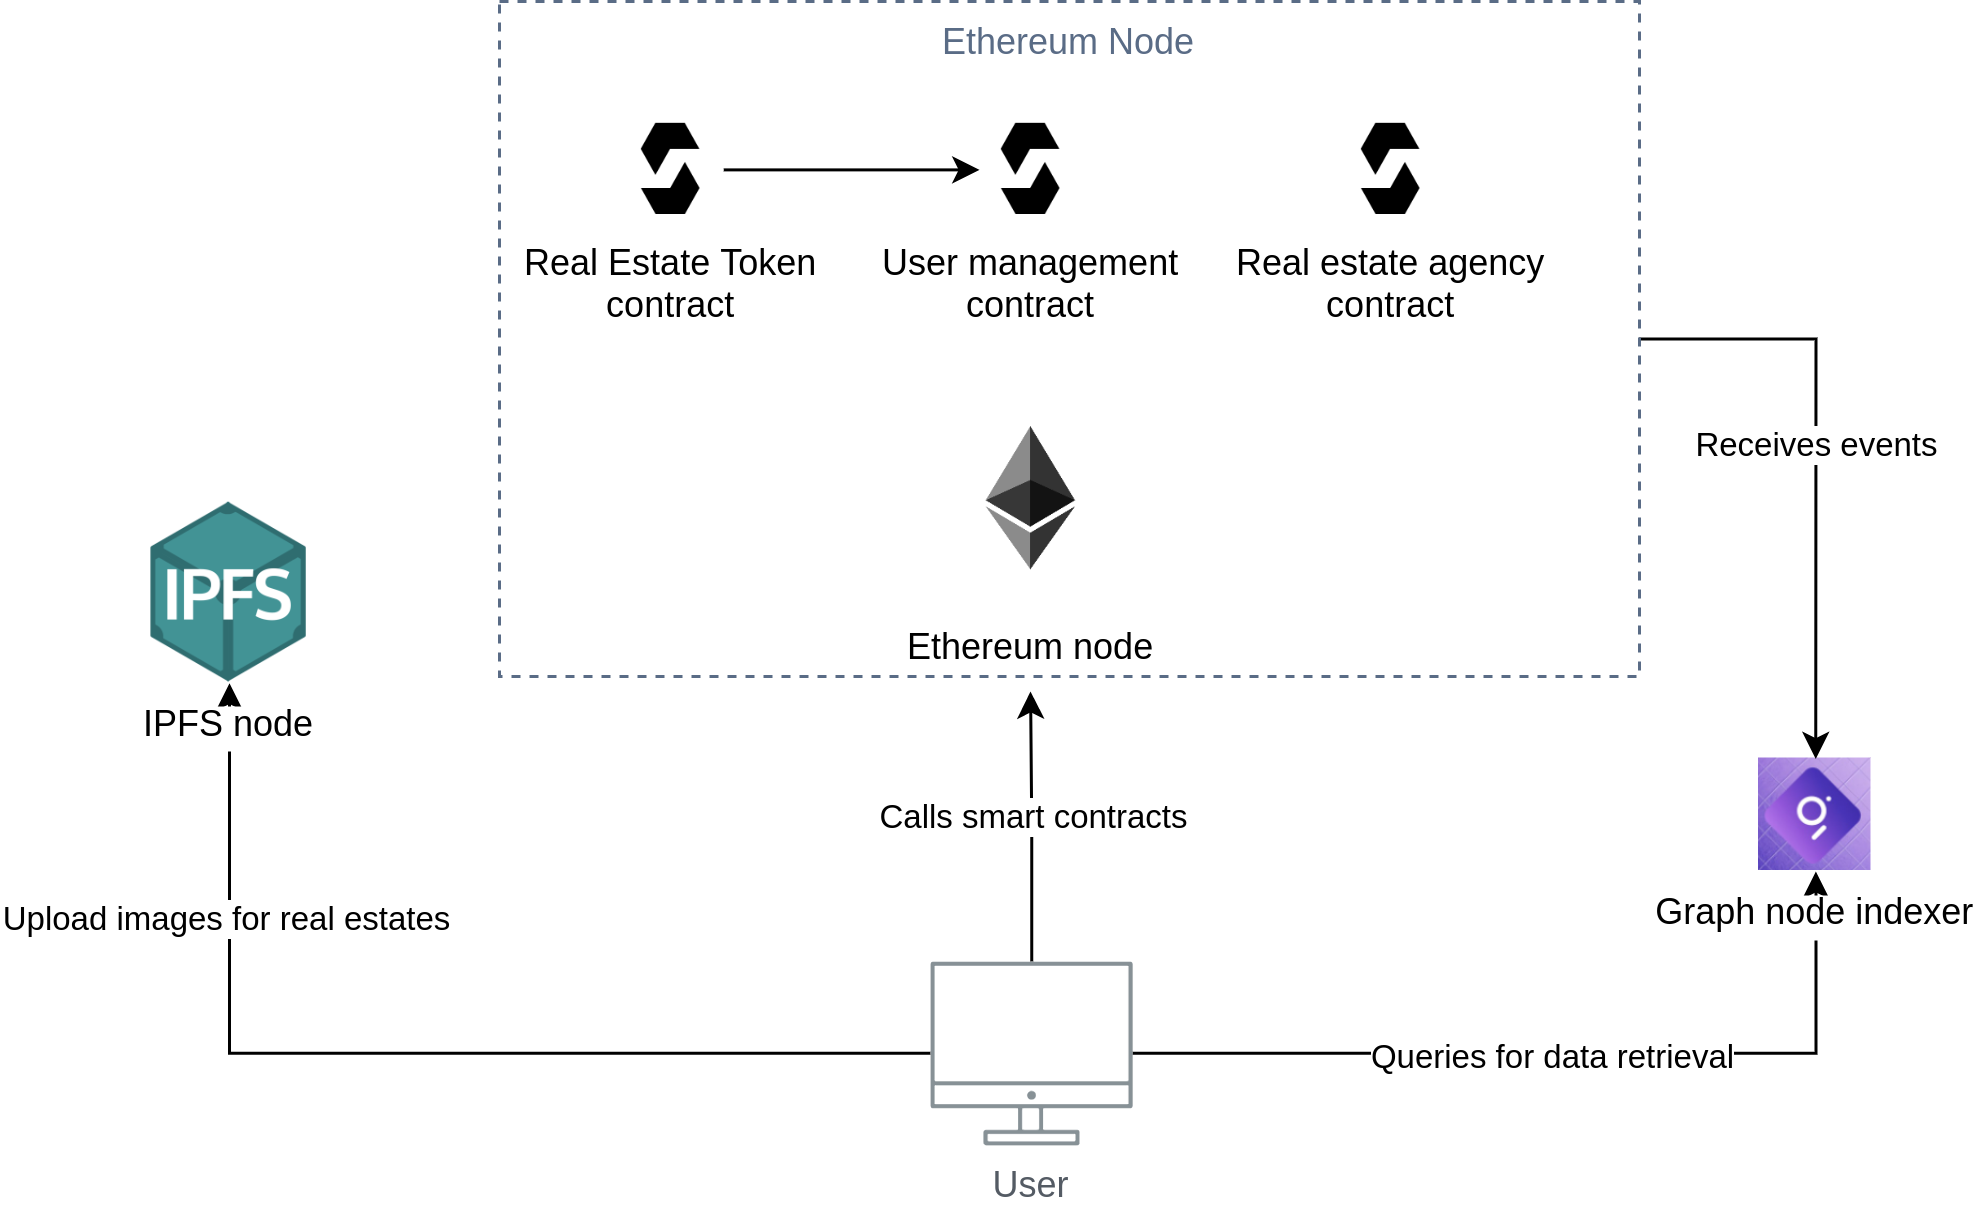
\includegraphics[width=\textwidth]{images/Real_Estate_arch.png}
    \fonte{Authors}
    \label{fig:application_architecture}
\end{figure}


\subsection{Real estate non-fungible token}

The real estate token smart contracts implement the Ethereum improvement proposal 721 (EIP-721) which is a standard for non-fungible tokens (NFTs).
Providing the core functionality to be implemented by a smart contract to track and transfer NFTs \cite{eip_721_2018}.
The NFT is used to represent the ownership of the real estates, having the metadata describing the property owned.

The creation of an NFT, also referred to as \textit{minting}, is not defined in the EIP-721. 
However, it's implemented in the smart contract and uses the user management contract to bind contact information about the owner of the asset.
The process of minting an NFT uses a role based access control (RBAC), having a minter role for this specific purpose.
Realtors have this role in order to register and manage real estates. 

Whenever a real estate is transferred, registered, sold, changed, events are created and processed by the Graph.
In order to support a better search mechanism, allowing users to search by places, price and trading options.

\begin{figure}[ht]
    \centering
    \caption{Real estate smart contract structure}
    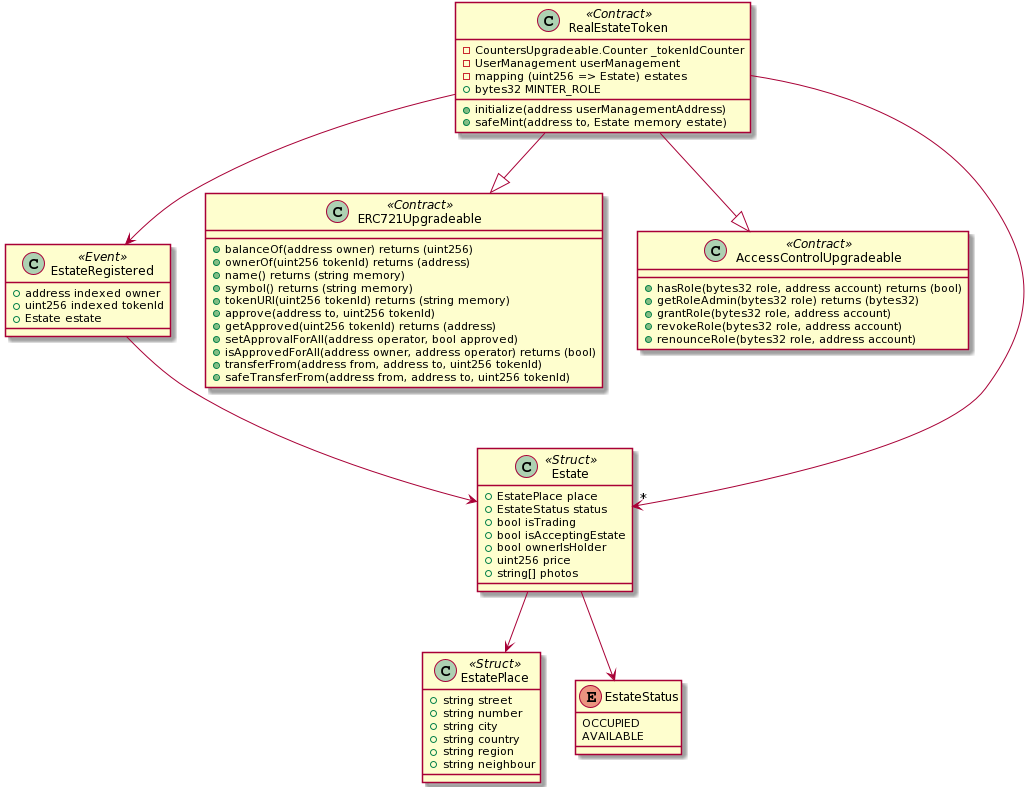
\includegraphics[width=\textwidth]{images/uml/real_estate_token.png}
    \fonte{Authors}
    \label{fig:real_estate_token_uml}
\end{figure}

Although it's considered expensive, the metadata is persisted on the blockchain for simplicity reasons of this project.
The ERC-721 standard defines the metadata URL as an external resource, not stored on blockchain, that may return a JSON content using a standard schema.
However, it's not used in this implementation.
The code implemented is small due to the usage of the base implementation of ERC-721 made by OpenZeppelin\footnote{https://docs.openzeppelin.com/contracts/4.x/erc721}.


\subsection{User management}

The user management contract allows users to sign up by providing their contact information, such as e-mail, cellphone.
The user can then be approved by a realtor, so that he can buy or own a real estate.
This contract has a RBAC system, having an approver role.

This contract is used by the real estate contract to register the owner of a given real estate.
There are events emitted when a user is registered, approved or denied.
Those events are processed by the Graph node mapping the user state to be queried by the Web application.

\begin{figure}[ht]
    \centering
    \caption{User management smart contract structure}
    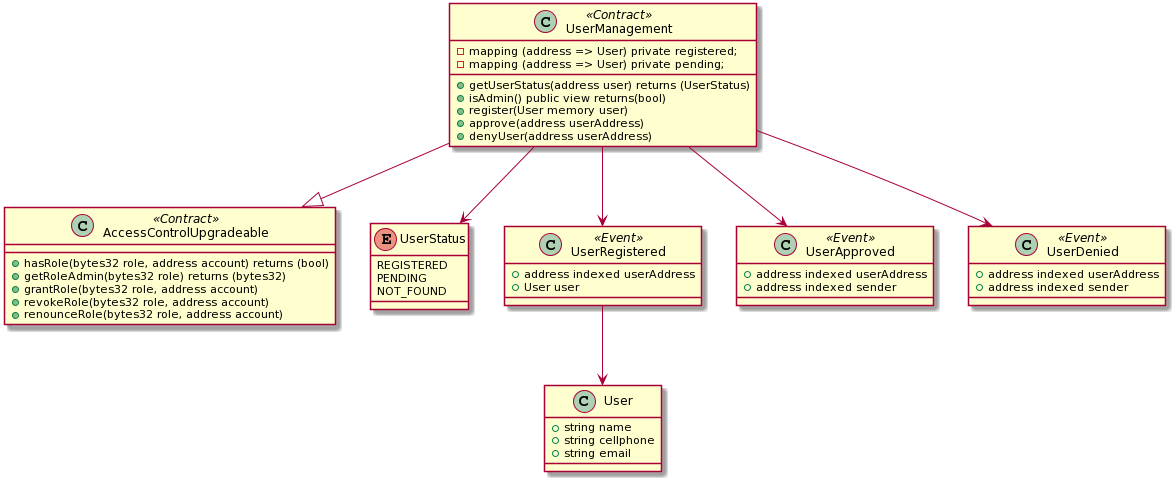
\includegraphics[width=\textwidth]{images/uml/user_management.png}
    \fonte{Authors}
    \label{fig:user_management_uml}
\end{figure}


\subsection{Web application}

The web application uses React as the main framework to construct the layout and the style of the pages, using the Redux library for the state management, global management of the application state.
In order to retrieve information about states with flexible queries, GraphQL protocol is used.
The Graph allows querying data with pagination, specific block hash or block number which allows time travel queries.

To support a better user experience, we use the Web3Modal\footnote{https://github.com/Web3Modal/web3modal} a library which supports multiple wallet providers, so users can choose their provider to use in the application.
The library supports Metamask, Dapper, Gnosis Safe, Frame, Web3 Browsers, and other providers that can be configured easily.

\begin{figure}[ht]
    \centering
    \caption{Web3 modal to select wallet provider}
    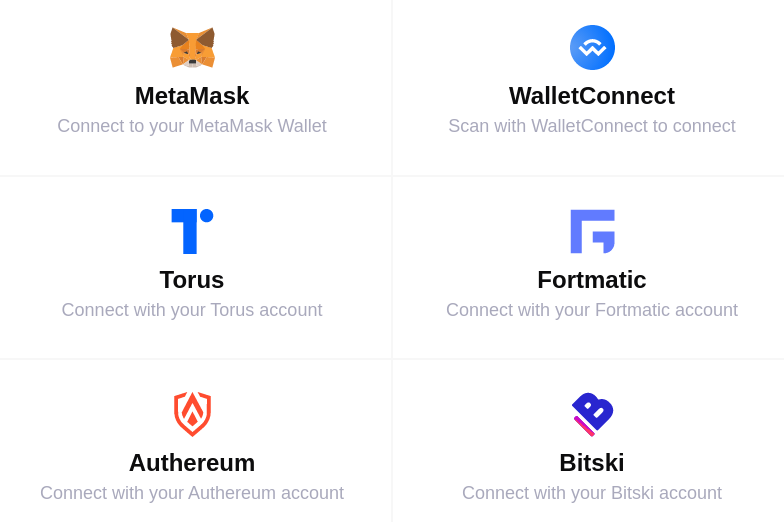
\includegraphics[width=350px]{images/web3_modal.png}
    \fonte{Reproduction}
    \label{fig:web3_modal}
\end{figure}


\section{Conclusion}

The Ethereum platform allows a new horizon of possible decentralized applications, beyond possible innovations such as decentralized autonomous organizations and non-fungible tokens.
There are multiple applications that implement the Ethereum standard among other features, which allows programmers and users to choose the best platform to execute the application.
By using applications such as IPFS, the Graph, it is possible to construct a solution only using Web 3 components.

The existing tools make the creation process of a decentralized application easier, having automated testing frameworks, automated deploys, possibility to test code locally and more.
The high-level programming language Solidity makes the process of coding a smart contract more easy, allowing modularity and a better reusability of the code by using the object-oriented concepts.


\bibliography{./references/abnt-template}

\end{document}
